\documentclass{article}


\usepackage{arxiv}

\usepackage[utf8]{inputenc} % allow utf-8 input
\usepackage[T1]{fontenc}    % use 8-bit T1 fonts
\usepackage{hyperref}       % hyperlinks
\usepackage{url}            % simple URL typesetting
\usepackage{booktabs}       % professional-quality tables
\usepackage{amsfonts}       % blackboard math symbols
\usepackage{nicefrac}       % compact symbols for 1/2, etc.
\usepackage{microtype}      % microtypography
\usepackage{lipsum}
\usepackage{siunitx}
\usepackage[linesnumbered,ruled,vlined]{algorithm2e}
\usepackage{float}
\usepackage{amsmath}
\usepackage{enumerate}
\usepackage{cite}
\usepackage{xcolor}
\usepackage{graphicx}
\graphicspath{ {../img/} }

\newcommand{\note}[1]{\textbf{#1}}

\title{Pratical Assignment: Solving PBO Problems with Evolutionary Algorithms}


\author{
 Xiang He\\
  s3627136\\
  \texttt{1234@umail.leidenuniv.nl}\\
  %% examples of more authors
   \And
 Shupei Li\\
  s3430863\\
  \texttt{s.li.18@umail.leidenuniv.nl} \\
  %% \And
 %% Name \\
  %% Student number\\
  %% \texttt{email address} \\
  %% \AND
  %% Coauthor \\
  %% Affiliation \\
  %% Address \\
  %% \texttt{email} \\
  %% \And
  %% Coauthor \\
  %% Affiliation \\
  %% Address \\
  %% \texttt{email} \\
  %% \And
  %% Coauthor \\
  %% Affiliation \\
  %% Address \\
  %% \texttt{email} \\
}

\begin{document}
\maketitle
%% \begin{abstract}
%% Abstract of your report here.
%% \end{abstract}


% keywords can be removed
%\keywords{First keyword \and Second keyword \and More}


\section{Introduction}\label{sec:intro}
% Intro: GA and ES
The evolutionary algorithm is one type of heuristic algorithm. It is inspired by the evolutionary process in nature and can be applied in various fields, such as engineering electrical electronics, automation control systems, etc \cite{2020slowik}. Generally, evolutionary algorithms begin with population initialization, which generates a set of individuals randomly. Then, the population is updated during the iteration until termination conditions are satisfied. Evolutionary algorithms guide the optimization direction via two basic operators, namely variation and selection \cite{2016eiben}. Variation includes recombination and mutation. It encourages the diversity of the population and a greater coverage of the search space. Selection consists of a series of evaluation strategies determining survivors during each epoch. It controls the overall quality of solution candidates and ensures the optimization does not deviate from the correct direction. The alternation between variation and selection simulates the gene inheritance and natural selection that balances between exploration and exploitation. In this assignment, we investigate two representative evolutionary algorithms --- the genetic algorithm and the evolution strategy. Specifically, we apply these two algorithms to solve two pseudo-boolean optimization (PBO) problems.

% F18
The domain of PBO problems is usually defined on $\{0, 1\}^n$, where $n$ represents the problem dimension. Meanwhile, the range of the problem is often limited on the field of real numbers $\mathbb{R}$. Given some constraints, our goal is finding a model satisfied $\{0, 1\}^n\rightarrow \mathbb{R}$ that maximizes (or minimizes) the objective function $F$. The first problem we aim to solve is the low autocorrelation binary sequences (LABS) problem. The input $\mathbf{s}$ of the LABS problem is usually defined on $\{-1, 1\}^n$. The objective of the LABS problem is:

\begin{align*}
    \min\ E\left( \mathbf{s} \right) = \sum_{k = 1}^{n - 1}\left( \sum_{i = 1}^{n - k} s_is_{i + k} \right)^2. 
\end{align*}

Or we can also maximize the merit factor equivalently, which is defined as:

\begin{align*}
    \max\ F\left( \mathbf{s} \right) = \frac{n^2}{2E\left( \mathbf{s} \right) }.
\end{align*}

The term $\frac{E(\mathbf{s})}{n}$ is the total energy of $n$ Ising spins $s_i\in\{-1, 1\}, i = 1, \dots, n$ in statistical physics \cite{2016packebusch}. Variants of the LABS problem have application value in fields like communication engineering and applied mathematics. However, our implementation transforms the domain into $\{0, 1\}^n$ to ensure the compatibility of the software environment. The final objective function can be written as:

\begin{align*}
    \max F(\mathbf{x}) &= \frac{n^2}{2 \sum_{k = 1}^{n - 1}\left(\sum_{i = 1}^{n - k} s_i\cdot s_{i + k}  \right)^2 }\\
    s.t.\quad s_i &= 2x_i - 1,\ x_i\in\{0, 1\}, i = 1, \dots, n.
\end{align*}

Figure \ref{fig:intro-labs} shows the largest known merit factors. Factors are confirmed to be optimal solutions when $n \leq 66$.

\begin{figure}[!ht]
 \begin{center}    
     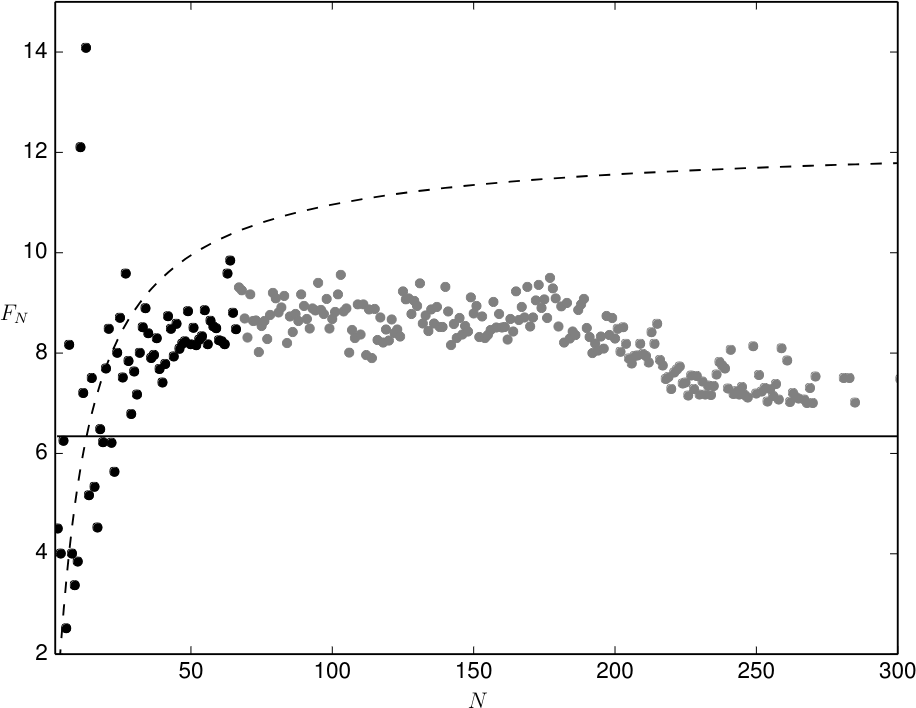
\includegraphics[width=0.5\textwidth]{labs.png}
 \end{center}
 \caption{Largest known merit factors (optimal when $n \leq 66$). This figure is directly adapted from \cite{2016packebusch}.}
 \label{fig:intro-labs}
\end{figure}

% F19
The second problem we focus on in this assignment is the Ising model. The Ising model is an NP-hard problem originating from the ferromagnetism theory. Its general form is defined on an undirected graph $G = \left( V, E \right) $. Each vertex in the graph corresponds to an Ising spin $s_i\in \{-1, 1\}$. Given a weight function $w$, the objective is maximizing $\sum_i\sum_j s_i\cdot s_j \cdot w(e_{ij})$, where $s_i, s_j\in V$ and $e_{ij}\in E$ \cite{2004briest}. In this assignment, we only consider the one-dimensional case, where the structure of the Ising model degenerates to a ring. With assumptions of zero
external magnetic fields and a unit interaction strength, the objective function of the Ising model is:

\begin{align*}
    \max\ F\left( \mathbf{x} \right) = \sum_{i, j, e_{ij}\in E} \left[ x_ix_j + \left( 1 - x_i \right)\left( 1 - x_j \right) \right].
\end{align*}

Notice that the similar transformation trick is applied: $x_i = \frac{s_i + 1}{2}, i = 1, \dots, n$. Consequently, the search space is mapped onto $\{0, 1\}^n$.

% ioh
Our algorithm implementation uses the IOHprofiler framework as the backbone. IOHprofiler integrates many benchmark problems and supports three types of analysis --- fixed-target, fixed-budget, and algorithm parameters \cite{2018doerr}. Two problems we study in this assignment have been added to IOHprofiler's built-in benchmark problems, denoted as F18 and F19 of the PBO class. With the help of the IOHprofiler, it is easy to build pipelines that automatically evaluate evolutionary algorithms' performance. We first record experimental logs via the IOHexperimenter module. After that, we upload logs to a free server running the IOHanalyzer service to obtain the statistical summary as well as results presented by images. All of results in this report are outputs of the IOHanalyzer.

% Structure
The rest of this report is organized as follows. Section \ref{sec:imple} describes the genetic algorithm and the evolution strategy in detail. It also provides information about hyperparameter settings. We report the metrics and experimental results in Section \ref{sec:experi}. This report ends with a brief conclusion and discussion.


\section{Algorithms}
\label{sec:imple}
\subsection{Genetic Algorithm}
\subsubsection{Overview}
The genetic algorithm is designed for the discrete search space, which usually appears in problems related to combinatorial optimization. The binary encoding is a common choice, i.e., $\mathbf{x}\in \{0, 1\}^n$. Given an objective function $F$, the outline of the genetic algorithm used in this project is shown in Algorithm \ref{al:ga-outline}.

\begin{algorithm}[!ht]
\SetAlgoLined
\SetKwInOut{Input}{Input}\SetKwInOut{Termination}{Termination}

\Input{Budget $B$, \\Problem dimension $n$, \\Population size $\mu$, \\Mutation rate $p_m$, \\Update ratio $\theta$, \\Objective function $F$, \\Tournament size $t_k$, \\Tournament probability $p_k$.}
\Termination{The algorithm terminates when $B \leq 0$.}
\SetKwFunction{FSelection}{Selection}
\SetKwFunction{FCrossover}{Crossover}
\SetKwFunction{FMutation}{Mutation}
\SetKwFunction{FEvaluation}{Evaluation}
\SetKwProg{Fn}{Function}{:}{}
\BlankLine

Initialize the population $\mathcal{D}^{(0)} = \{\mathbf{x}_1, \mathbf{x}_2, \dots, \mathbf{x}_{\mu}\}$ by random sampling, where $\mathbf{x}_i = \left[ x_1, x_2, \dots, x_n \right]^T, i = 1,\dots, \mu$ and $x_j\sim \text{iid}\ \texttt{Bernoulli}\left( 0.5 \right), j = 1, \dots, n$\;
\FEvaluation{$\mathcal{D}^{(0)}$, $F$, $B$}\;
$B_{copy}$ = $B$\;

\BlankLine
\While{$B > 0$}{
    updateNumber = $\mu\cdot \theta$\;
    \tcc{Update the population partially.}
    \While{updateNumber $> 0$}{
        $p_1$, $p_2$ = \FSelection{$\mathcal{D}^{(t)}$, $B$, $B_{copy}$, $t_k$, $p_k$}\;
        $c$ = \FCrossover{$p_1$, $p_2$}\;
        \FEvaluation{$c$, $F$, $B$}\;
        \If{c.fitness > $\mathbf{x}_1$.fitness}{
            Delete $\mathbf{x}_1$ from $\mathcal{D}^{(t)}$\;
            $\mathcal{D}^{(t)}$ = $\mathcal{D}^{(t)}$ $\cup$ $c$\;
            Sort $\mathcal{D}^{(t)}$ in ascending order according to fitness values\;
        }
    }
    \FMutation{$\mathcal{D}^{(t)}$, $p_m$}\;
    \FEvaluation{$\mathcal{D}^{(t)}$, $F$, $B$}\;
    $\mathcal{D}^{(t + 1)} = \mathcal{D}^{(t)}$
}

\BlankLine
\Fn{\FEvaluation{$\mathcal{D}$, $F$, $B$}}{
    \For{$i = 1$ \KwTo $\mathcal{D}$.size}{
        $\mathbf{x}_i$.fitness = $F\left( \mathbf{x}_i \right) $\;
        $B$ = $B$ - 1\;
    }
    Sort $\mathcal{D}$ in ascending order according to fitness values\;
}
\caption{Overview of Genetic Algorithm}\label{al:ga-outline}
\end{algorithm}

In the vanilla genetic algorithm, offspring are generated by applying the selection, crossover, and mutation operators sequentially at time $t$. Then, the population at time $t + 1$ is a copy of these offspring. However, we found that updating the whole population at each time step often leads to an unstable performance in pilot experiments. The reason is that the overall population quality may decrease during the optimization since there is no guarantee that offspring have higher fitness values than parents. A decline in the population quality caused by offspring generation is not a big problem with a sufficient budget and a relatively small problem dimension. The decrease in quality at the early stage usually means a broader exploration area in search space and can be compensated easily later. But given $B = 5,000$ and $n = 50$, the convergence rate of the vanilla genetic algorithm is too slow to find a satisifying solution when the budget runs out. To overcome this weakness, we improve the vanilla genetic algorithm in several aspects:

\begin{itemize}
    \item Introduce a hyperparameter update ratio $\theta$ to control the proportion of updating population at each time step. $\theta = 1$ corresponds to the vanilla genetic algorithm, while $\theta = \frac{1}{\mu}$ means only update one individual.
    \item Maintain the ascending order of the population based on the fitness value. An offspring will only be by added to the population if its fitness value is better than the first individual's.
    \item Design a hybrid selection strategy that will be described in Section \ref{subsubsec:selection}. Outputs of the selection operator are two individuals set as parents.
    \item Use an inner loop to generate the offspring one by one until the update ratio is satisfied at each time step, aiming at saving budget and encouraging diversity.
\end{itemize}

The following three sections introduce selection, crossover, and mutation operators used in Algorithm \ref{al:ga-outline} in detail.

\subsubsection{Selection}\label{subsubsec:selection}
There are various selection strategies for the genetic algorithm. The different strategies put different selection pressures on the population during optimization. Here, we mainly consider three representative selection strategies and develop a hybrid selection operator. Algorithm \ref{al:ga-selection} illustrates the idea of combining different selection strategies.

\begin{algorithm}[!ht]
\SetAlgoLined
\SetKwProg{Fn}{Function}{:}{}
\SetKwFunction{FSelection}{Selection}
\SetKwFunction{FPropSelection}{ProportionalSelection}
\SetKwFunction{FRankSelection}{RankSelection}
\SetKwFunction{FTourSelection}{TournamentSelection}
\BlankLine

\Fn{\FSelection{$\mathcal{D}$, $B$, $B_{copy}$i, $t_k$, $p_k$}}{
    $B_{current}$ = $B_{copy} - B$\;
    \uIf{$B_{current} < (0.4\ast B_{copy})$}{
        \FPropSelection{$\mathcal{D}$}\tcp*{Early stage: proportional selection.}
    }
    \uElseIf{$B_{current} < (0.6 \ast B_{copy})$}{
        \FRankSelection{$\mathcal{D}$}\tcp*{Middle stage: rank selection.}
    }
    \Else{
        \FTourSelection{$\mathcal{D}$, $t_k$, $p_k$}\tcp*{Late stage: tournament selection.}
    }
    Sample two individuals $p_1, p_2$ without replacement from $\mathcal{D}$ by simple random sampling, where $P(\mathbf{x}\text{ is selected}) = \mathbf{x}$.p\_selection\;
    \Return{$p_1, p_2$}
}

\BlankLine
\Fn{\FPropSelection{$\mathcal{D}$}}{
    sum = 0\;
    \ForEach{$\mathbf{x}\in\mathcal{D}$}{
        sum = sum + $\mathbf{x}$.fitness\;
    }
    \ForEach{$\mathbf{x}\in\mathcal{D}$}{
        $\mathbf{x}$.p\_selection = $\mathbf{x}$.fitness / sum\;
    }
}

\BlankLine
\Fn{\FRankSelection{$\mathcal{D}$}}{
    \tcc{$\mathcal{D}$ is sorted based on fitness.}
    \For{$i = 1$ \KwTo $\mathcal{D}$.size}{
        $\mathbf{x}_i$.p\_selection = $(2\ast i) / (\mathcal{D}.\text{size}\ast (\mathcal{D}.\text{size} + 1))$\;
    }
}

\BlankLine
\Fn{\FTourSelection{$\mathcal{D}$, $t_k$, $p_k$}}{
    Sample $t_k$ individuals from $\mathcal{D}$ to constitute $\mathcal{D}_{tour}$. For other non-selected individuals, $\mathbf{x}$.p\_selection = 0\;
    Sort $\mathcal{D}_{tour}$ in descending order according to fitness values\;
    \For{$i = 1$ \KwTo $\mathcal{D}_{tour}$.size}{
        $\mathbf{x}_i$.p\_selection = $p_k(1 - p_k)^i$\;
    }
    Normalize the selection probabilities.\;
}
\caption{Genetic Algorithm: Hybrid Selection Operator}\label{al:ga-selection}
\end{algorithm}

Proportional selection assigns a selection probability to each individual that is proportional to the fitness. The intuition behind this strategy is the survival of the fittest. However, the proportional selection is likely affected by significant variations in $F$, which may lead to the local optimum trap. Rank selection is a selection strategy that is more robust to the variance. It decides selection probabilities based on a function of the ranking. Here, we adopt the ranking function suggested by \cite{2012cs}:

\begin{align*}
    P\left( \mathbf{x}_i\text{ is selected} \right) = \frac{2r_i}{\mu(\mu + 1)}.
\end{align*}

where $r_i$ is the rank of the individual $x_i$ based on its fitness value in ascending order, and $\mu$ is the population size. Tournament selection is another commonly used strategy. Given a pre-defined tournament size $t_k$ and the tournament probability $p_k$, it firstly samples $t_k$ individuals from the population. Then, the selected individuals compete for the parent qualification following the Geometric distribution with the success probability equal to $p_k$. In other words, the $i$-th fittest individual is assigned the selection probability $p_k\left( 1 - p_k \right)^i $. We apply the normalization to all individuals at the end of the tournament to ensure the sum of selection probabilities equals 1.

The selection pressure of proportional selection, rank selection, and tournament selection increases sequentially. High selection pressure encourages exploitation and reduces exploration, and vice versa. Therefore, we divide the optimization into three stages to balance between exploitation and exploration. The hybrid selection operator can be summarized as follows:

\begin{enumerate}
    \item Early stage: current budget $>$ 0.6 $\times$ total budget. Use the proportional selection to explore the search space.
    \item Middle stage: 0.4 $\times$ total budget $\leq$ current budget $<$ 0.6 $\times$ total budget. Use the rank selection to shift from exploration to exploitation.
    \item Late stage: current budget $\leq$ 0.4 $\times$ total budget. Use the tournament selection to exploit current optimal solutions.
\end{enumerate}

\subsubsection{Crossover}
We choose the one-point crossover operator in the genetic algorithm. Algorithm \ref{al:ga-crossover} and Figure \ref{fig:al-ga-crossover} show the logic of this operator.

\begin{algorithm}[!ht]
\SetAlgoLined
\SetKwProg{Fn}{Function}{:}{}
\SetKwFunction{FCrossover}{Crossover}
\BlankLine
\Fn{\FCrossover{$p_1, p_2$}}{
    Generate a random integer $m \in \{1, 2, \dots, p_1.\text{length}\} $\;
    $c = p_1[:m] + p_2[m + 1:]$\;
    \Return{c}
}
\caption{Genetic Algorithm: One-point Crossover Operator}\label{al:ga-crossover}
\end{algorithm}

\begin{figure}[!ht]
 \begin{center}    
     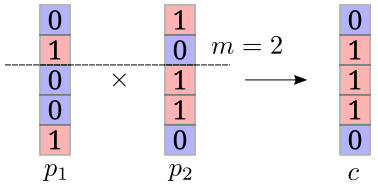
\includegraphics[width=0.5\textwidth]{ga/ga-crossover.png}
 \end{center}
 \caption{One-point crossover operator. Assume $m = 2$.}
 \label{fig:al-ga-crossover}
\end{figure}

Inputs of crossover operator are two parents $p_1 = \left[x_1, x_2, \dots, x_n \right]^T$ and $p_2 = \left[ y_1, y_2, \dots, y_n \right]^T$. The crossover point is generated by sampling an integer $m\in\{1, 2, \dots, n\}$. The child $c$ is produced by swapping bits between parents based on the crossover point, that is, $c = \left[x_1, \dots, x_m, y_{m + 1}, \dots, y_n  \right]^T $. Traditionally, the crossover operator will output two children. However, we only retain the first child because we update the population partially in the genetic algorithm. Redundant offspring will waste valuable budgets.

\subsubsection{Mutation}
The mutation operator introduces variations into solutions to broaden the search area in the feasible region. We adopt the bit flip mutation operator because of the usage of binary encoding. The bit flip mutation operator is illustrated in Algorithm \ref{al:ga-mutation} and Figure \ref{fig:al-ga-mutation}.

\begin{algorithm}[!ht]
\SetAlgoLined
\SetKwProg{Fn}{Function}{:}{}
\SetKwFunction{FMutation}{Mutation}
\BlankLine
\Fn{\FMutation{$\mathcal{D}$, $p_m$}}{
    \ForEach{$\mathbf{x}\in\mathcal{D}$}{
        \For{i = 1 \KwTo $\mathbf{x}$.length}{
            Sample $d \sim \texttt{Uniform}(0, 1)$\;
            \If{$d < p_m$}{
                $x_i$ = $|x_i - 1|$\;
            }
        }
    }
}
\caption{Genetic Algorithm: Bit Flip Mutation Operator}\label{al:ga-mutation}
\end{algorithm}

\begin{figure}[!ht]
 \begin{center}    
     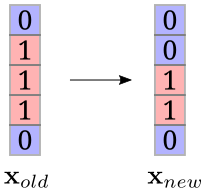
\includegraphics[width=0.28\textwidth]{ga/ga-mutation.png}
 \end{center}
 \caption{Bit flip mutation operator. Assume the second location of the individual is flipped.}
 \label{fig:al-ga-mutation}
\end{figure}

The mutation operator is applied to the whole population. For each location of the individual, the bit flipping happens with probability $p_m$, i.e., $0\rightarrow 1, 1 \rightarrow 0$. With mutation, we can increase the diversity of solutions.

\subsubsection{Hyperparameter Settings}
There are three major hyperparameters in the genetic algorithm --- population size $\mu$, mutation rate $p_m$, and update ratio $\theta$. We perform hyperparameter fine-tuning on these parameters with the grid search method. The fine-tuning results are discussed in Section $\ref{sec:experi}$. As for other hyperparameters, we determine their values according to assignment requirements and the results of pilot experiments. Table \ref{tab:al-ga-hyper} summarizes the hyperparameter settings of the genetic algorithm for reproducibility.

\begin{table}[!ht]
    \centering
    \caption{Hyperparameter settings of the genetic algorithm.}
    \label{tab:al-ga-hyper}
    \begin{tabular}{lll}
       \toprule
       \textbf{Hyperparameter} & \textbf{Meaning} & \textbf{Value}\\
       \midrule
       $B$ & budget & 5,000\\
       $n$ & problem dimension & 50\\
       $t_k$ & tournament size & Equal to the population size\\
       $p_k$ & tournament probability & 0.8\\
       \bottomrule
    \end{tabular}
\end{table}

We set the random seed to 42 when running the genetic algorithm.

\subsection{Evolution Strategy}


\section{Experimental Results}\label{sec:experi}
\subsection{Metrics}

\subsection{Genetic Algorithm}
\subsubsection{Fine-tuning: Population Size}

\subsubsection{Fine-tuning: Mutation Rate}

\subsubsection{Fine-tuning: Update Ratio}

\subsubsection{Final Results}

\subsection{Evolutionary Strategy}


\section{Discussion and Conclusion}
\label{sec:dis&res}
% TODO: Remember to write the future work.

\bibliographystyle{unsrt}  
\bibliography{references}  

\end{document}
